\documentclass[]{article}
\usepackage{lmodern}
\usepackage{amssymb,amsmath}
\usepackage{ifxetex,ifluatex}
\usepackage{fixltx2e} % provides \textsubscript
\ifnum 0\ifxetex 1\fi\ifluatex 1\fi=0 % if pdftex
  \usepackage[T1]{fontenc}
  \usepackage[utf8]{inputenc}
\else % if luatex or xelatex
  \ifxetex
    \usepackage{mathspec}
  \else
    \usepackage{fontspec}
  \fi
  \defaultfontfeatures{Ligatures=TeX,Scale=MatchLowercase}
\fi
% use upquote if available, for straight quotes in verbatim environments
\IfFileExists{upquote.sty}{\usepackage{upquote}}{}
% use microtype if available
\IfFileExists{microtype.sty}{%
\usepackage{microtype}
\UseMicrotypeSet[protrusion]{basicmath} % disable protrusion for tt fonts
}{}
\usepackage[margin=1in]{geometry}
\usepackage{hyperref}
\hypersetup{unicode=true,
            pdftitle={Standardization \& Balancing PrintTree plugin},
            pdfauthor={Cristina Muschitiello~Food and Agriculture Organization of the United Nations},
            pdfkeywords={Commodity Tree, FBS, CPC, shares, extraction Rates, conversion factors},
            pdfborder={0 0 0},
            breaklinks=true}
\urlstyle{same}  % don't use monospace font for urls
\usepackage{graphicx,grffile}
\makeatletter
\def\maxwidth{\ifdim\Gin@nat@width>\linewidth\linewidth\else\Gin@nat@width\fi}
\def\maxheight{\ifdim\Gin@nat@height>\textheight\textheight\else\Gin@nat@height\fi}
\makeatother
% Scale images if necessary, so that they will not overflow the page
% margins by default, and it is still possible to overwrite the defaults
% using explicit options in \includegraphics[width, height, ...]{}
\setkeys{Gin}{width=\maxwidth,height=\maxheight,keepaspectratio}
\IfFileExists{parskip.sty}{%
\usepackage{parskip}
}{% else
\setlength{\parindent}{0pt}
\setlength{\parskip}{6pt plus 2pt minus 1pt}
}
\setlength{\emergencystretch}{3em}  % prevent overfull lines
\providecommand{\tightlist}{%
  \setlength{\itemsep}{0pt}\setlength{\parskip}{0pt}}
\setcounter{secnumdepth}{5}
% Redefines (sub)paragraphs to behave more like sections
\ifx\paragraph\undefined\else
\let\oldparagraph\paragraph
\renewcommand{\paragraph}[1]{\oldparagraph{#1}\mbox{}}
\fi
\ifx\subparagraph\undefined\else
\let\oldsubparagraph\subparagraph
\renewcommand{\subparagraph}[1]{\oldsubparagraph{#1}\mbox{}}
\fi

%%% Use protect on footnotes to avoid problems with footnotes in titles
\let\rmarkdownfootnote\footnote%
\def\footnote{\protect\rmarkdownfootnote}

%%% Change title format to be more compact
\usepackage{titling}

% Create subtitle command for use in maketitle
\newcommand{\subtitle}[1]{
  \posttitle{
    \begin{center}\large#1\end{center}
    }
}

\setlength{\droptitle}{-2em}
  \title{Standardization \& Balancing\\
\texttt{PrintTree} plugin}
  \pretitle{\vspace{\droptitle}\centering\huge}
  \posttitle{\par}
  \author{Cristina Muschitiello~Food and Agriculture Organization of the United
Nations}
  \preauthor{\centering\large\emph}
  \postauthor{\par}
  \predate{\centering\large\emph}
  \postdate{\par}
  \date{12 June 2018}

\usepackage{lscape}
\usepackage{booktabs}
\usepackage{longtable}
\usepackage{array}
\usepackage{multirow}
\usepackage[table]{xcolor}
\usepackage{wrapfig}
\usepackage{float}
\usepackage{colortbl}
\usepackage{pdflscape}
\usepackage{tabu}
\usepackage{threeparttable}
\usepackage{threeparttablex}
\usepackage[normalem]{ulem}
\usepackage{makecell}

\usepackage{draftwatermark}
\usepackage{makeidx}
\makeindex
\usepackage{float}
\floatplacement{figure}{H}
\usepackage{amsmath}
\usepackage{amssymb}
\usepackage{amsthm}
\usepackage{mathtools}
\usepackage{caption}

\begin{document}
\maketitle
\begin{abstract}
This vignette provides a description of the \texttt{printTree} plug-in:
This plug-in has been created for creating a document will all the
tables of the Standardization and Balancing together, by
country-year-FBScommodity.
\end{abstract}

{
\setcounter{tocdepth}{4}
\tableofcontents
}
\newpage

\listoftables

\listoffigures

\subsection*{Disclaimer}\label{disclaimer}
\addcontentsline{toc}{subsection}{Disclaimer}

This Working Paper should not be reported as representing the official
view of the FAO. The views expressed in this Working Paper are those of
the author and do not necessarily represent those of the FAO or FAO
policy. Working Papers describe research in progress by the authors and
are published to elicit comments and to further discussion.

This paper is dynamically generated on \today{} and is subject to
changes and updates.

\newpage

\section{Introduction}\label{introduction}

The process of combining commodity balances for creating Food Balance
Sheets is explained in a separate document\footnote{see Standardization
  \& Balancing for Food Balance Sheet Calculation}. The process is based
on a structured and clear set of relationships between commodity given
by the \emph{Commodity tree} which is also explained in another
document. The \emph{Standardization and Balancing} generates balances
for FBS commodities at different levels of aggregation: by FBS item, by
group, by family and Total (by country). The \texttt{printTree} plug-in
performs the all process (as the
\texttt{Full\ standardization\ and\ balancing\ does}) but only for a
single FBS item's SUA. It saves the different outputs, plus some detail
about commodity tree, extraction rates and shares in a .md file and send
it to the user for easy consultation.

One of the main drawbacks of the structure of plug-ins and processes in
the SWS for FBSs calculation is the fact of having pieces of information
separated in different data-tables and data-sets. This makes it a bit
complicated for a user to have the full picture of a country when is
trying to validate a Food Balance Sheet. For this reason, a tool has
been created for having slices of country information in a single
document. Indeed, the complexity of the Food Balance Sheet makes it not
possible to have all pieces of information together. In particular, FBSs
have many dimensions: countries, FBS commodities, years, SUAs. Also,
there are many ways of looking at the data: by country, by year, by FBS
commodity by step of the process and so on.

The SWS shows the data in data-sets representing different step of the
process. These data-sets are ordered by country, commodity and year.
This structure is not the best in many cases fr a user. The
\texttt{printTree} plug-in shows, for a selected FBS item, country and
year, the different tables in a unique document.

\section{Content (the output of the
plug-in)}\label{content-the-output-of-the-plug-in}

The output of the plug-in is a \texttt{.md} file that is better red by
\emph{Notepad ++}. The name of the document is:

\texttt{year\_M49\_sample\_test.md}, for example:
\texttt{2014\_1248\_sample\_test.md}, where 1248 is the M49 code for
China Mainland. It is composed the following parts:

\subsection{\texorpdfstring{\texttt{sua\_unbalanced}}{sua\_unbalanced}}\label{sua_unbalanced}

First, the \texttt{Sua\ Unbalanced} if shown for the FBS item selected.
In the example of figure \ref{fig:f1} The Sua for the FBS item
\emph{WHEAT \& PRODUCTS} is shown. This means that all the CPC
commodities of the Commodity Tree of Wheat are shown, plus the
commodities that will be aggregated in the FBS item \emph{WHEAT \&
PRODUCTS} but are NOT in the commodity Tree of Wheat: \emph{Food
PReparations} and \emph{Mixes and dougths}\footnote{a more detailed
  description of the commodities included in the sua\_unbalanced table
  is contained in the methodological document of \emph{Standardization
  and Balancing}}.

\subsection{\texorpdfstring{\texttt{sua\_unbalanced\ +\ Production\ filled}}{sua\_unbalanced + Production filled}}\label{sua_unbalanced-production-filled}

The first step of the Sua Filling is the creation/increment of
production for derived commodities. The overall process is described in
the methodological document of Standardization and Balancing.

The result of this step is reported in the second part of the printTree
document (figure \ref{fig:f2}). Any change from the previous table is
reported with 3 asterisk (***) before and after.

\newpage

\begin{landscape}
\begin{figure}[H]

{\centering 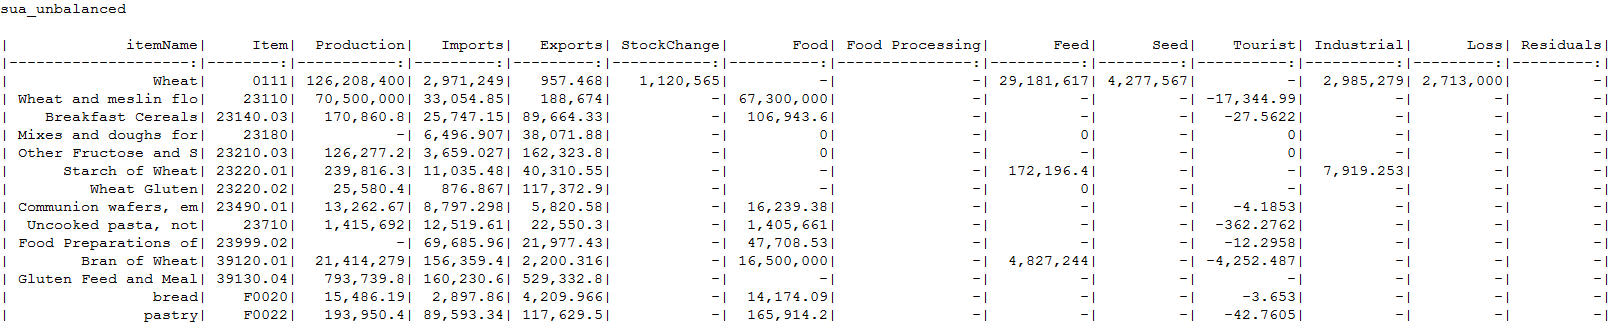
\includegraphics[width=1\linewidth]{images/printTree/01_unbalanced} 

}

\caption{\label{fig:f1}printTree output 1 - sua unbalanced}\label{fig:f1}
\end{figure}

\begin{figure}[H]

{\centering 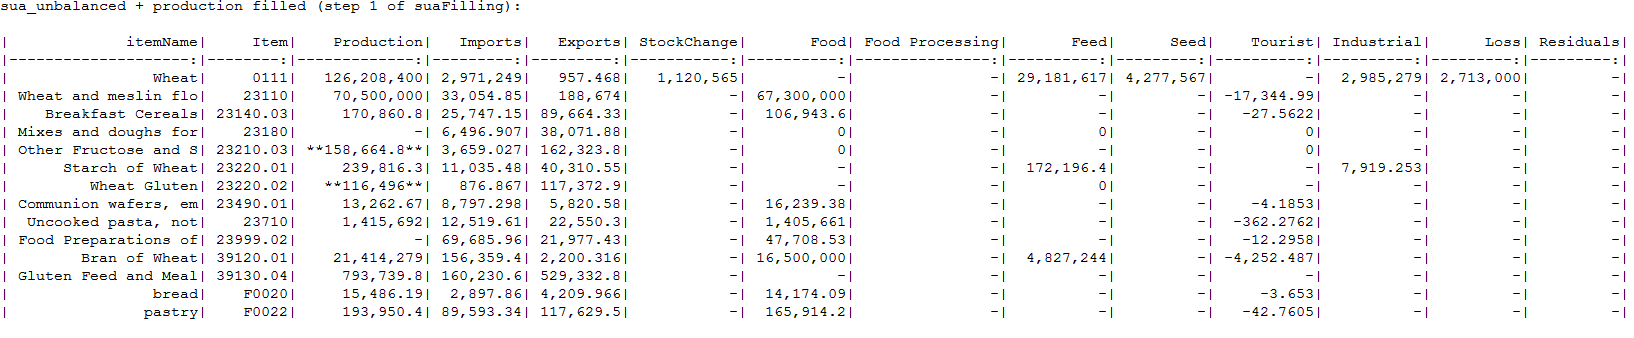
\includegraphics[width=1\linewidth]{images/printTree/02_unbalanced2} 

}

\caption{\label{fig:f2}printTree output 2 - sua unbalanced with production}\label{fig:f2}
\end{figure}
\end{landscape}

\subsection{Availabilities, extraction rates and shares for Food
Processing
calculation}\label{availabilities-extraction-rates-and-shares-for-food-processing-calculation}

The document includes the table with extraction Rates, shares, weights
and availabilities (figure \ref{fig:f3}) used for the next step, which
is the calculation of Food Processing. Please notice that here, not just
the portion of commodity tree of Wheat is reported, but also any other
related commodity. In particular, with \emph{related} commodity is meant
that, if a child of the commodity tree of wheat, is also child of dome
other commodity of some other tree, also this commodity is reported,
because is related to that child of wheat. This additional commodity
will be also shown in the next steps because its figures might change,
and actually change, when the figure of the FBS wheat tree change.

\begin{figure}[H]

{\centering 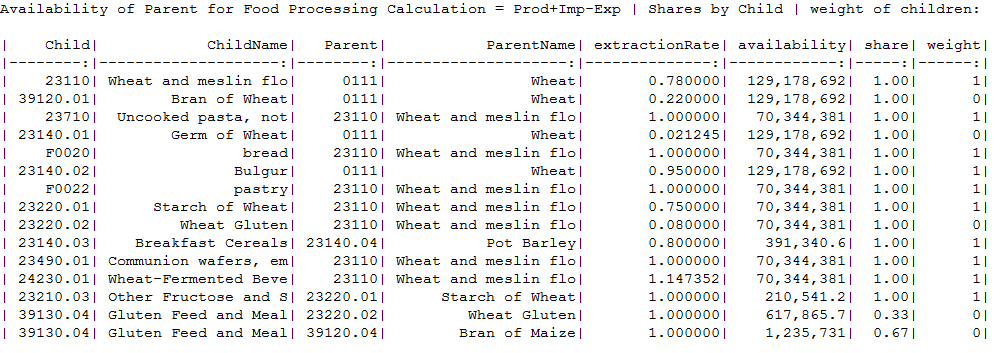
\includegraphics[width=0.9\linewidth]{images/printTree/03_availabilities} 

}

\caption{\label{fig:f3}printTree output 3 - availabilities, extraction rates and shares for Food Processing calculation}\label{fig:f3}
\end{figure}

\subsection{\texorpdfstring{\texttt{sua\_unbalanced\ +\ Production\ filled\ +\ Food\ Processing}}{sua\_unbalanced + Production filled + Food Processing}}\label{sua_unbalanced-production-filled-food-processing}

From table in figure \ref{fig:f3}, Food processing (\ref{fig:f24}) can
be better understood. Also in figure \ref{fig:f4} Any change from the
previous table is reported with 3 asterisk (***) before and after.

\subsection{\texorpdfstring{\texttt{sua\_balanced} and Nutrient
Values}{sua\_balanced and Nutrient Values}}\label{sua_balanced-and-nutrient-values}

After food processing, the sua filling compute/change any other figure
that is required. The result is the sua\_unbalanced table (figure
\ref{fig:f4}). The table also reports the DES (Dietary Energy Supply).
Indeed, as described in the methodological document, DES is based on
food quantities at this step of the process.

\newpage

\begin{landscape}
\begin{figure}[H]

{\centering 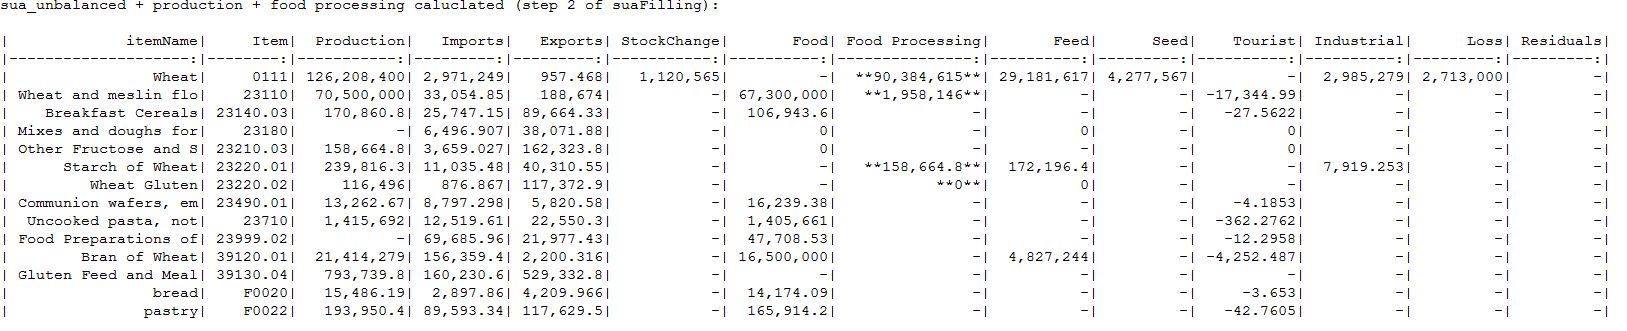
\includegraphics[width=1\linewidth]{images/printTree/04_unbalanced3} 

}

\caption{\label{fig:f4}printTree output 4 - sua unbalanced with Food Processing}\label{fig:f4}
\end{figure}

\begin{figure}[H]

{\centering 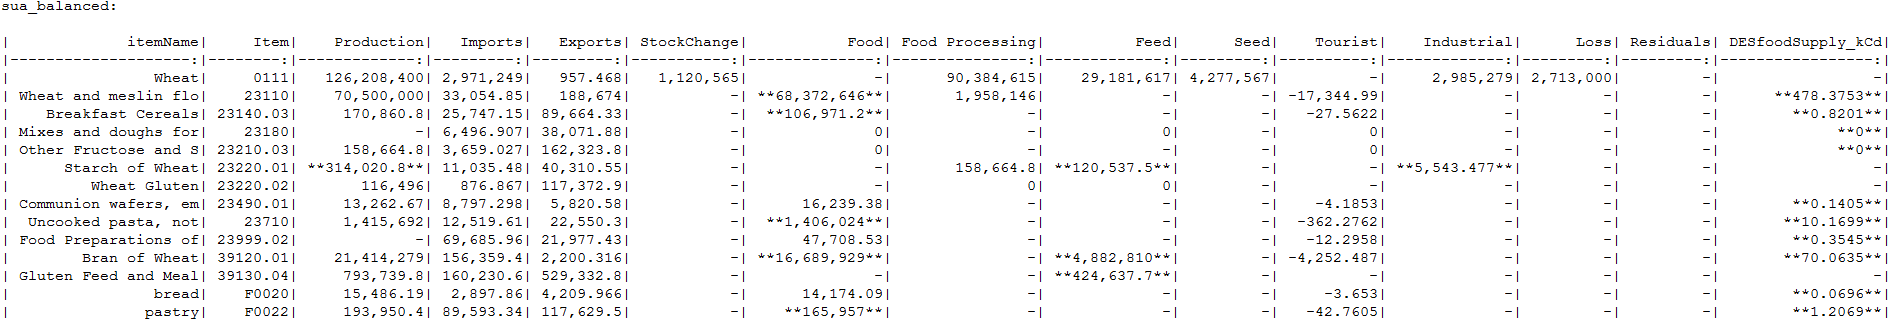
\includegraphics[width=1\linewidth]{images/printTree/05_balanced} 

}

\caption{\label{fig:f5}printTree output 5 - sua balanced (after Sua Filling)}\label{fig:f5}
\end{figure}
\end{landscape}

\subsection{Availabilities, extraction rates and shares for
Standardization}\label{availabilities-extraction-rates-and-shares-for-standardization}

Also for Standardization, a table extracted from the commodity tree is
reported, with Availability, extraction rates, shares and weights. Also
in this case, \emph{related} commodities are shown.

\begin{figure}[H]

{\centering 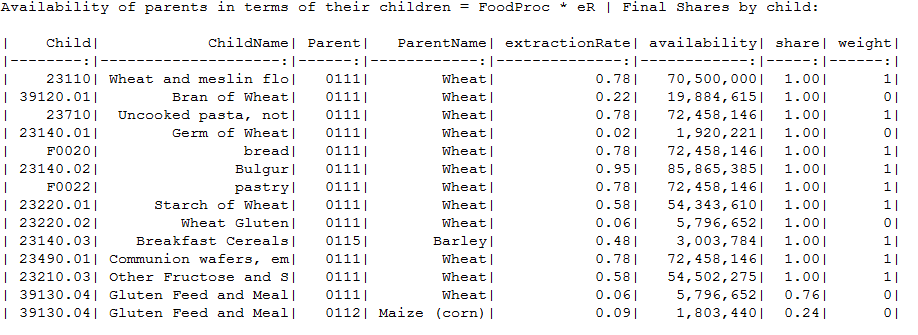
\includegraphics[width=0.9\linewidth]{images/printTree/06_availability2} 

}

\caption{\label{fig:f6}printTree output 6 - availabilities, extraction rates and shares for standardization}\label{fig:f6}
\end{figure}

\subsection{\texorpdfstring{\texttt{fbs\_standardized}}{fbs\_standardized}}\label{fbs_standardized}

figure \ref{fig:f7} shows the result of standardization. Only zero-level
commodities are reported in this table. Again any change from the
previous table is reported with 3 asterisk (***) before and after.

\subsection{\texorpdfstring{\texttt{fbs\_balanced} and adjustment of
Nutrient
Values}{fbs\_balanced and adjustment of Nutrient Values}}\label{fbs_balanced-and-adjustment-of-nutrient-values}

Two tables are reported for balanced Food Balance Sheet. One for the
quantities (figure \ref{fig:f8}) and one with the Nutrient values
updated (figure \ref{fig:f9}).

\subsection{FBS aggregation}\label{fbs-aggregation}

Finally, all the FBS item aggregated are reported. Also related FBS
items are reported. Tables reported in figure \ref{fig:f9} contain all
level of aggregations.

All the tables presented are contained in a single document.

\newpage

\begin{landscape}
\begin{figure}[H]

{\centering 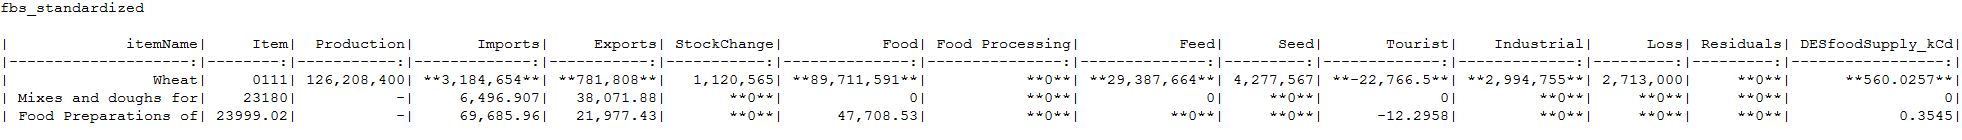
\includegraphics[width=1\linewidth]{images/printTree/07_standardized} 

}

\caption{\label{fig:f7}printTree output 7 - fbs standardized}\label{fig:f7}
\end{figure}

\begin{figure}[H]

{\centering 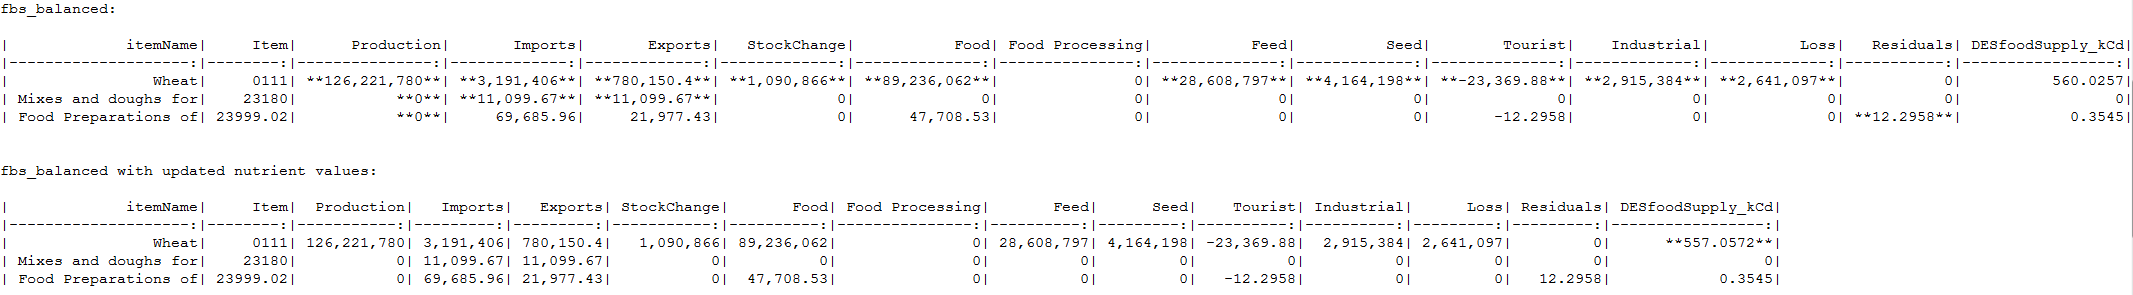
\includegraphics[width=1\linewidth]{images/printTree/08_balanced_nutrients} 

}

\caption{\label{fig:f8}printTree output 8 - fbs balanced and fbs balanced with nutrients updated}\label{fig:f8}
\end{figure}

\begin{figure}[H]

{\centering 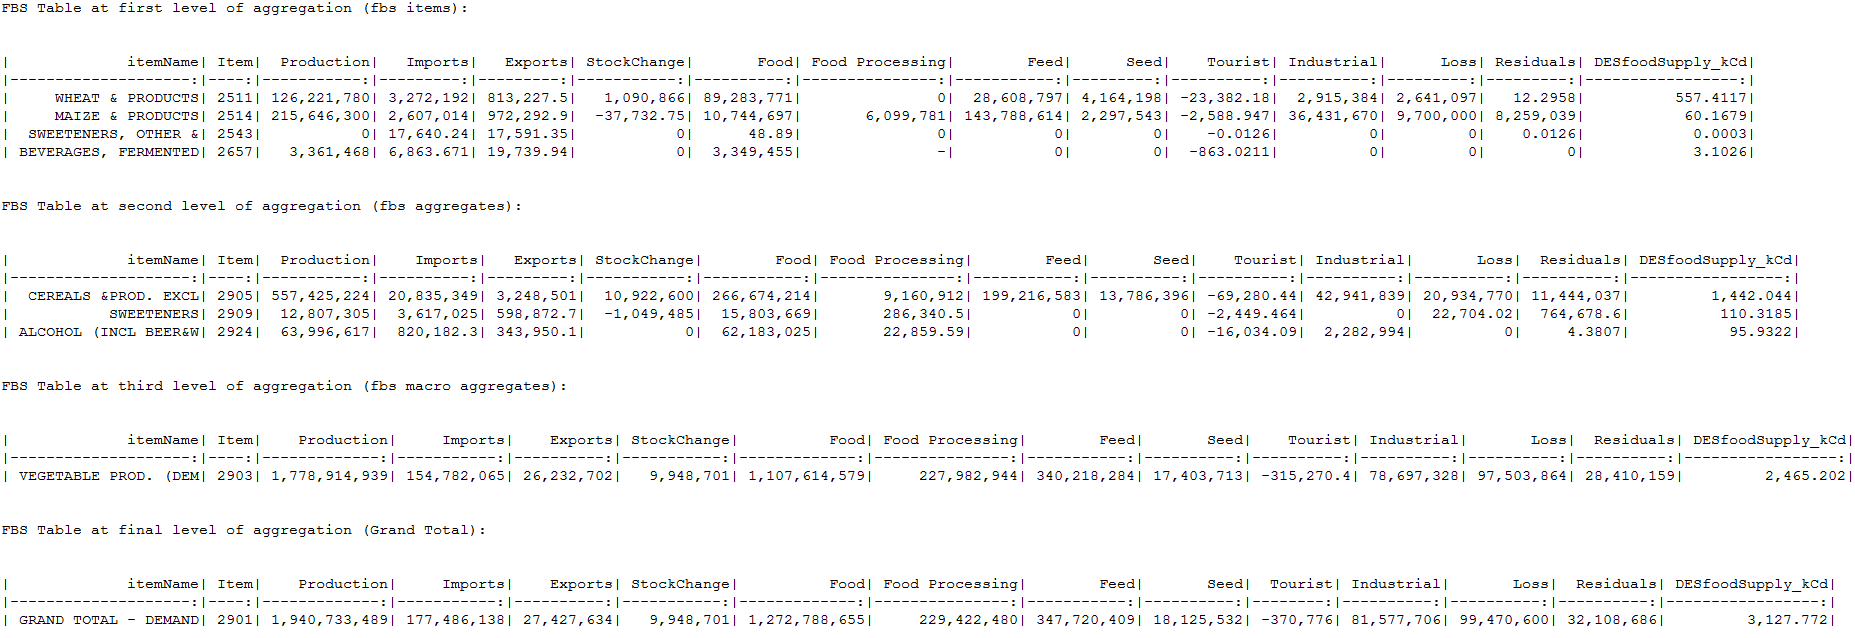
\includegraphics[width=1\linewidth]{images/printTree/09_aggregations} 

}

\caption{\label{fig:f9}printTree output 9 - FBS aggregations}\label{fig:f9}
\end{figure}
\end{landscape}

\section{\texorpdfstring{\texttt{printTree}
Plug-in}{printTree Plug-in}}\label{printtree-plug-in}

\subsection{Input dataset}\label{input-dataset}

The plug-in is selected and launched from the \texttt{sua\_unbalanced}
data-set. Therefore, a session has to be opened in this data-set (figure
\ref{fig:f10}). From the session, the \emph{R plugins} section has to be
opened and the \texttt{printTree} plug-in selected (figure
\ref{fig:f11}).

\begin{figure}[H]

{\centering 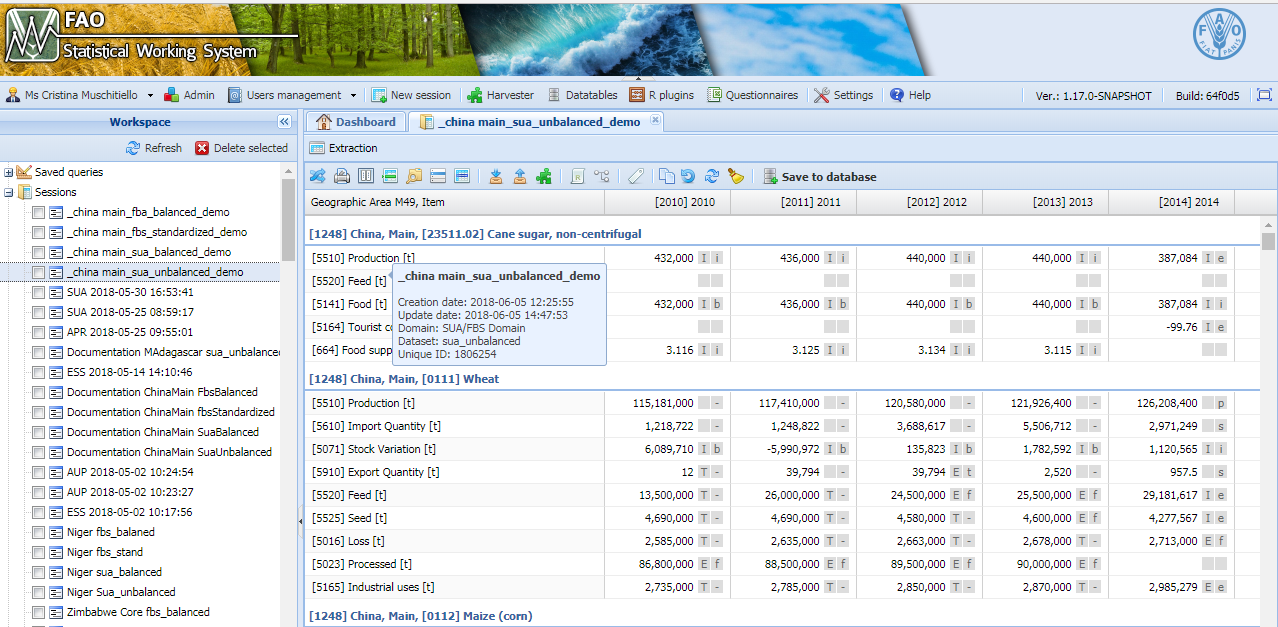
\includegraphics[width=1\linewidth]{images/printTree/10_inputSession} 

}

\caption{\label{fig:f10}printTree plug-in: input dataset}\label{fig:f10}
\end{figure}

\subsection{Plug-in definition}\label{plug-in-definition}

\begin{figure}[H]

{\centering 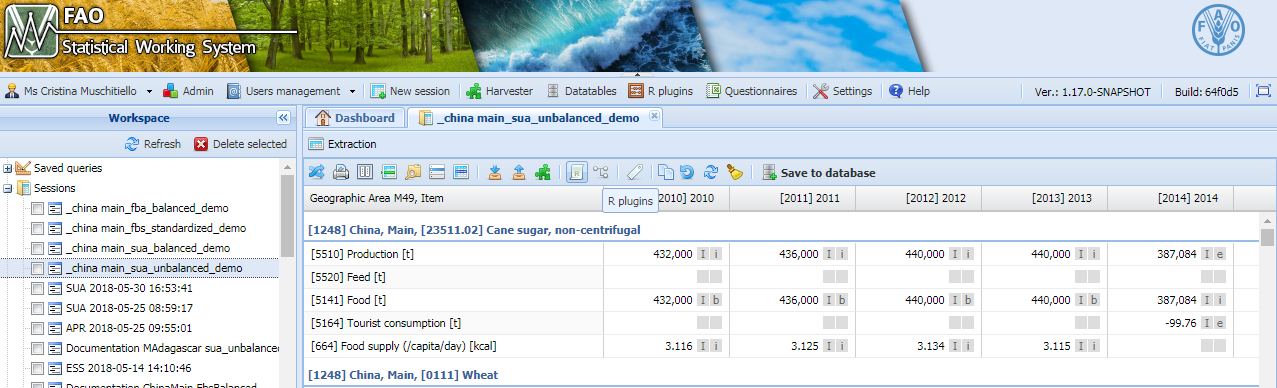
\includegraphics[width=1\linewidth]{images/printTree/11_runbotton} 

}

\caption{\label{fig:f11}printTree plug-in: call plug-in window }\label{fig:f11}
\end{figure}

Figure \ref{fig:f12} shows the drop-down menu for the selection of the
FBS item. Also first and last year have to be selected and the
countries. Always \emph{session country} is selected in this case
(figure \ref{fig:f13}).

\begin{figure}[H]

{\centering 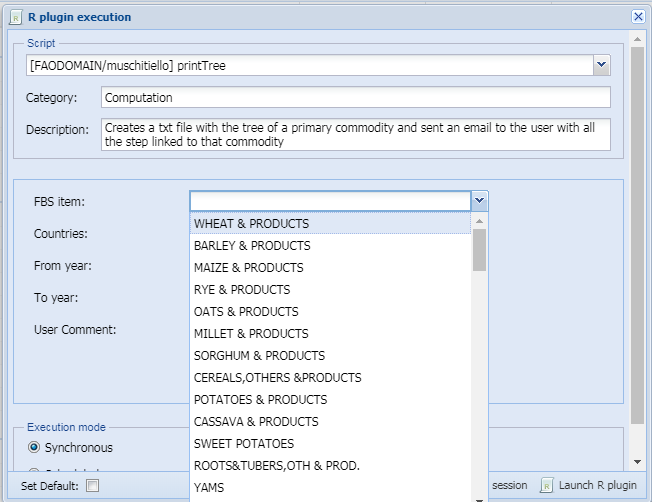
\includegraphics[width=0.8\linewidth]{images/printTree/12_selectfbs} 

}

\caption{\label{fig:f12}printTree plug-in: select FBS item from drop down menu}\label{fig:f12}
\end{figure}

\begin{figure}[H]

{\centering 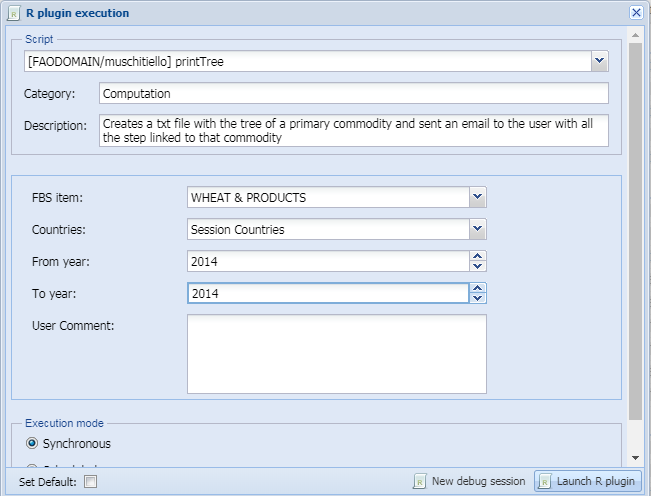
\includegraphics[width=0.8\linewidth]{images/printTree/13_launch} 

}

\caption{\label{fig:f13}printTree plug-in: select other parameters and run}\label{fig:f13}
\end{figure}

\subsection{Plug-in output}\label{plug-in-output}

When the plug-in has run, an email is sent with an attached folder
(figure \ref{fig:f14}). The folder includes other folder before reaching
the file. This is due to the structure of the SWS server and for the
moment is not possible to simplify this structure (figure
\ref{fig:f15}). Finally the file is contained, the content of which has
been already explained. It has to be opened with \emph{Notepad ++}.

\begin{figure}[H]

{\centering 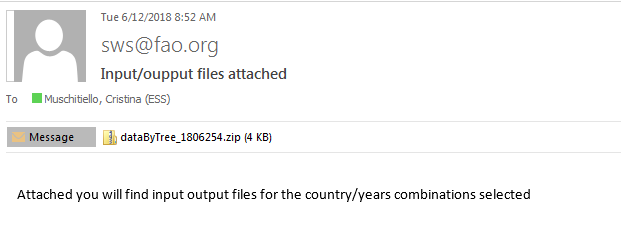
\includegraphics[width=0.8\linewidth]{images/printTree/14_messageEmail} 

}

\caption{\label{fig:f14}printTree plug-in: email}\label{fig:f14}
\end{figure}

\begin{figure}[H]

{\centering 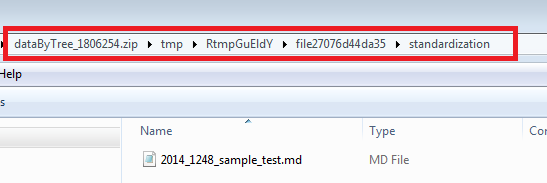
\includegraphics[width=0.8\linewidth]{images/printTree/15_emailContent} 

}

\caption{\label{fig:f15}printTree plug-in: folders}\label{fig:f15}
\end{figure}


\end{document}
